% define rectangle
\tikzstyle{block} = [draw, rectangle, 
    minimum height=3em, minimum width=3em]
    \tikzstyle{Cir} = [draw, circle, 
    minimum size=0.5em]

\usetikzlibrary{shapes.multipart}    
\tikzset{
state/.style={
       rectangle split,
       rectangle split parts=2,
       rectangle split part fill={green!20,red!20},
       rounded corners=0.1cm,
       draw,
       %draw=black, very thick,
       minimum height=3em, minimum width=3em,
       %text width=3cm,
       %inner sep=2pt,
       text centered,
       }
}    
    
   
\tikzstyle{input} = [coordinate]
\tikzstyle{output} = [coordinate]
\tikzstyle{pinstyle} = [pin edge={to-,thin,black}]
\tikzset{fontscale/.style = {font=\Huge}
    }
\begin{figure}
        \centering
        
        
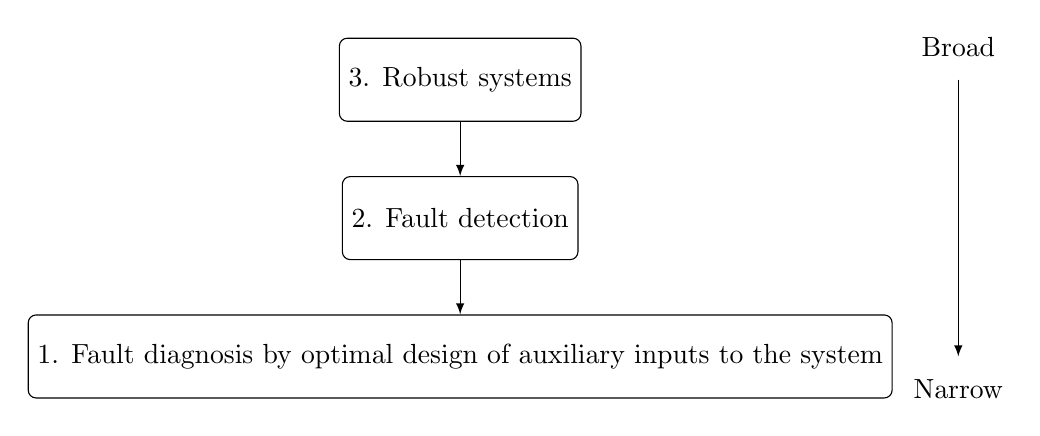
\begin{tikzpicture}[node distance=0em, >=latex] 
    \node [input, name=input]  {};
    \node [block, fill=white!20, rounded corners=0.1cm, align=center, yshift=0em, below of=input] (lvl1)  {3. Robust systems};
    \node [block, fill=white!20, rounded corners=0.1cm, align=center, yshift=-5em, below of=lvl1] (lvl2)  {2. Fault detection};
    \node [block, fill=white!20, rounded corners=0.1cm, align=center, yshift=-5em, below of=lvl2] (lvl3)  {1. Fault diagnosis by optimal design of auxiliary inputs to the system};
    \node [input, name=narrow, below of=lvl3, xshift=18em] {Narrow};
    \node [input, name=broad, below of=lvl1, xshift=18em] {Broad};
   
      
    \draw [draw,->] (lvl1) -- node [near start, above = 1em] {} (lvl2);
    \draw [draw,->] (lvl2) -- node [near start, above = 1em] {} (lvl3);
    \draw [draw,->] (broad) -- node [near start, above = 3em] {Broad} node [near end, below= 3em] {Narrow} (narrow);
\end{tikzpicture}
 
 
        \caption{Different levels of the motivation displayed from broad to narrow.}
        \label{tikz:diagram}
\end{figure}